\documentclass[12pt]{article}
\usepackage[a4paper, margin=.30in]{geometry}
\usepackage{graphicx ,
            wrapfig,
            xcolor, 
            enumerate,
            amsmath,fontenc,
            tcolorbox,mathrsfs
            }
\usepackage{mathptmx}
\usepackage[siunitx, RPvoltages]{circuitikz}
\newcommand\headerMe[2]{\noindent{}#1\hfill#2}
\renewcommand{\thesection}{\Roman{section}}

\author{Zakaria HAOUZAN}
\date{\today}

\begin{document}
% headers --------------
\headerMe{Matière : Physique-Chimie}{Professeur : Zakaria HAOUZAN}\\
\headerMe{Unité : Electricité}{Établissement : Lycée SKHOR qualifiant}\\
\headerMe{Niveau : 1BAC-SM/X}{Heure : 12H/6H}\\

% ------Content ________

%\begin{wrapfigure}[10]{r}{0.5\textwidth}
    %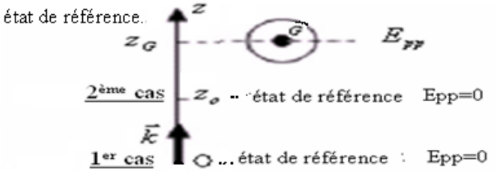
\includegraphics[width=0.5\textwidth]{./img/img00.png}
%\end{wrapfigure}


%\begin{tcolorbox}[colback=black!15!white,
                  %colframe=black!10!black,
                  %title=Remarque :
                 %]
\begin{center}

    \Large{Leçon $N^{\circ} 8 $: \color{red}Transfert de l’énergie dans un circuit électrique- Puissance
électrique. }
\end{center}

%\begin{wrapfigure}[10]{r}{0.3\textwidth}
  %\vspace{-1cm}
    %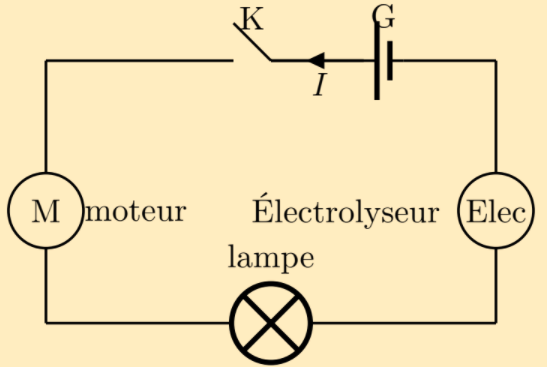
\includegraphics[width=0.3\textwidth]{./img/img_00.png}
%\end{wrapfigure}


\section{Rappel :  }
  \subsection{Tension et intensité du courant dans un circuit électrique }
On considère le montage électrique suivant, qui est formé par un
générateur de tension G et trois conducteurs ohmiques . On donne
$R1 = 47\Omega$ , $R2 = 33\Omega$ , U1 = 6V et U = 9V.
Trouver la valeur de la résistance R3 en expliquant la méthode
utilisée.

  %\begin{circuitikz}[]
%%    \draw (0,0) -- (4,0)--(4,4)--(0,4) -- cycle;
  %%\draw (0,0) rectangle (8,8);
  %%\draw (0,0) parabola (8,8);
  %%\draw (4,4) .. controls (4,8) and (8,4) .. (8,8);
  %%\draw (4,4) circle (6cm);
  %%\draw (2,2) ellipse (3cm and 1cm);
  %%\draw[step=1cm,gray,very thin] (-2,-2) grid (8,8.9);
  %%\draw[very thick, ->] (0, 0) --(5,0);
  %%\draw[thick, ->] (0, 0) --(0,5);

    %\draw (0,0) to[vsource, v=$V_0$ ] (0,3) -- (2,3)
 %to[R] (2,0) -- (0,0);
%\end{circuitikz}
  %\begin{circuitikz}[american]
    %\draw (1,0) to[isource, l=$I_0$] (1,3) --(2,3)
    %to[R=$R_1$](2,0)--(1,0);

    %\draw (2,3)--(5,3) to[R=$r_2$] (5,0) -- (1,0);
  %\end{circuitikz}
  \begin{center}
  \begin{circuitikz}[european, voltage shift=0.5]
    \draw (0,6)
    to[battery1, v=$U$, i=$I$] (6,6)
    to[short](6,3)
    to[R, name=R1,v=$U_1$] (3,3)
    to[short, ](3,4)
    to[R=$R_2$, v=$U_2$](1,4)
    to[short ](1,3)
    to[short](0,3)--(0,6)
    ;
    \draw (3,3)
    to[short] (3,2)
    to[R=$R_3$] (1,2)--(1,3)
    ;
    \node at (R1.center) {$R_1$};
  \end{circuitikz}
  \end{center}
\subsection{Le courant électrique : }
On définit un courant électrique par la quantité d’électricité qui
traverse une section S d’un conducteur électrique au cours de la
durée $\Delta{t}$ :$$I=\frac{Q}{\Delta{t}}$$
Q : La quantité d’électricité exprimée en coulomb C et $\Delta$t la durée
du temps en seconde (s) et I est l’intensité du courant exprimée en
ampère (A) .

Le sens conventionnel du courant électrique est le sens contraire
du déplacement des électron dans un conducteur .
On mesure l’intensité du courant électrique à l’aide d’un
\textbf{ ampèremètre }.

\begin{tcolorbox}
  Pour mesurer l’intensité du courant dans une branche de circuit à
l’aide d’ampèremètre qui se branche en série dans la branche .
\begin{circuitikz}[ european, voltage shift=0.5]
  \draw (0,0) to[R, name=R1,i=I](4,0) to[ammeter](6,0);
  \node at (R1){R};
\end{circuitikz}
\end{tcolorbox}

\subsection{La tension électrique : }
La tension électrique entre deux points A et B d’un circuit ou la
différence de potentielle $U_{AB} = V_A-V_B$ est une grandeurs
algébrique qui se mesure à l’aide d’un voltmètre .
Le voltmètre se branche en dérivation entre les deux point A et
B .

\begin{circuitikz}[ european, voltage shift=0.5]
  \draw (-0.5,0)node{COM}(0,0) 
  to[voltmeter, name=v] ++(4,0) 
  (4.2,0)node {+} 
  (4,0) to[short](4,2)

  (0,2)to[R,name=R1,i=I](4,2)
  (0,2) to[short](0,0)
  ;
  %\node (R.center){R1};
\end{circuitikz}

\section{Introduction : }
Les plaques solaires de cette maison reçoivent une énergie de
rayonnement qui la transforme en énergie électrique ou thermique
( chauffage de l’eau , éclairage,..)
\\Quelles sont les expressions de l’énergie et de la puissance
électrique reçues ? 
\\Quels sont les différentes transferts ou
transmissions d’énergies qui se font au niveau des récepteurs ? et
qu’est ce que l’effet joule ?

\section{Transfert d’énergie au niveau d’un récepteur
électrique}
\begin{wrapfigure}[10]{r}{0.3\textwidth}
  \vspace{-2cm}
    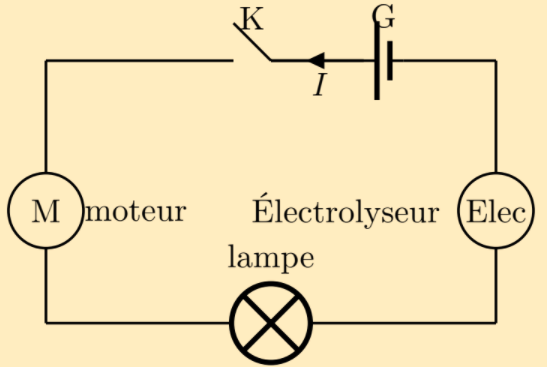
\includegraphics[width=0.3\textwidth]{./img/img_00.png}
\end{wrapfigure}


\subsection{Définition et exemples de récepteurs électriques}
\subsubsection{Activité 1 : }
On réalise le montage électrique suivant et qui est formé par un
générateur branché en série avec une lampe , un moteur
électrique, un interrupteur K et un électrolyseur .
\\1-On ferme l’interrupteur K , que se passe -t-il au niveau de chaque
dipôle ?
\\2-Quelles sont les formes d’énergie qui sont produit par
chaque dipôle ?
\\3-Qu’il est le dipôle électrique qui fournit de l’énergie au
reste de circuit ?
\\4-Qu’appelle-t-on les dipôles électriques suivants : la lampe ;
le moteur et l’électrolyseur ?

\subsubsection{Exploitation}
Lorsqu’on ferme le circuit on observe :
\\ *la lampe brille et chauffe.
\\ * l’électrolyseur est le siège de réactions chimiques au niveau de
chaque électrode
\\ * Le moteur tourne .
\vspace{.2cm}

2 -Les formes d’énergie qui se produit par chaque dipôle sont :
\\ * dans la lampe : énergie calorifique et énergie de
rayonnement ;
\\ * dans le moteur : énergie calorifique et énergie mécanique ;
\\ * dans l’électrolyseur : énergie calorifique et énergie chimique
\vspace{.2cm}

3-Le générateur qui fournit de l’énergie électrique nécessaire
pour faire fonctionner les éléments de circuit électrique.

4-Ce sont des récepteurs électriques

\subsubsection{Définition :}
Un récepteur électrique est un dipôle qui convertit l’énergie
électrique reçue en une autre forme d’énergie
\begin{wrapfigure}[3]{r}{0.3\textwidth}
    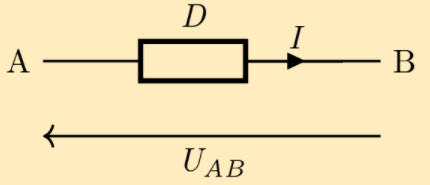
\includegraphics[width=0.3\textwidth]{./img/img_01.png}
\end{wrapfigure}


\subsection{Puissance électrique reçue par un récepteur :}
\underline{Dipôle en convention récepteur} 
: $U_{AB}$ est positif si le sens de
courant est de A vers B .

\underline{Le régime permanent :}Lorsqu’on ferme un circuit électrique, le fonctionnement
régulier (uniforme) des élément du circuit nécessite une
certaine durée . Après cette durée , on dit que les récepteurs
fonctionnent en régime permanent.

\subsection{Puissance électrique reçue par un récepteur : }
En régime permanent et en courant continue , la puissance $\mathscr{P}_e$
transférée à un récepteur est égale au produit de la tension $U_{AB}$ à
ses bornes par l’intensité du courant qui le traverse :
\fbox{$\mathscr{P}_e = U_{AB}.I$}
\\$\mathscr{P}_e$ s’exprime en watt (W) .$ U_{AB}$ en volt et I en ampère (A) .
\subsection{Énergie électrique reçue par un récepteur}
Par définition une puissance est définie comme le quotient du
travail par $\Delta{t}$ du transfert :
$$\fbox{
  $\mathscr{P} = \frac{W}{\Delta{t}}$
}$$
De façon analogue , la puissance électrique reçue par un récepteur
pendant une durée $\Delta{t}$ est :
$$\fbox{
  $\mathscr{P} = \frac{W_e}{\Delta{t}}$
}$$
D’où We l’énergie électrique reçue par récepteur pendant la durée
$\Delta{t}$ :
$W_e = \mathscr{P}.\Delta{t}$
$$\fbox{
  $
W_e = U_{AB}.I.\Delta{t} 
$
}\;\;(1)
$$

\begin{tcolorbox}
L’unité dans SI de l’énergie électrique est le joule (J).
On utlise une autre unité d’énergie , c’est le kWh
$$1kWh = 1000×3600 = 3,6.10^6J$$
\end{tcolorbox}

\begin{tcolorbox}[colback=black!15!white,
                  colframe=black!10!black,
                  title=Remarque :
                 ]
Pour une même énergie électrique transférée , la puissance
transférée est d’autant plus grande que la durée de temps du
transfert est faible.
  \\La puissance électrique $\mathscr{P}e$ permet d’évaluer la rapidité d’un
transfert d’énergie . Donc la puissance est la vitesse du transfert
d’énergie .

\end{tcolorbox}

\begin{tcolorbox}[colback=blue!15!white,
                  colframe=blue!50!black,
                  title=Application 1 :
                 ]
Un moteur fonctionnent sous une tension de 9V , reçoit une
  puissance de 1,5W pendant une durée de $\Delta{t}$ = 2,0min .
\\1. Calculer le travail électrique reçu par le moteur
\\2. En déduire l’intensité du courant qui le traverse .
\end{tcolorbox}

\section{Effet Joule}

\subsection{Définition}
Lorsqu’un courant électrique traverse un fil conducteur , il
s’échauffe . On appelle cet effet thermique du courant électriqueL’
effet joule
\\L’effet joule est l’effet thermique associé au passage du courant
électrique dans un conducteur . Il se manifeste sous deux formes :
transfert sous forme thermique et par rayonnement.
\\Ce phénomène est nommé par effet Joule relativement au savant
Britannique JAMES PRESCOTT JOULE (1818-1889)

\subsection{Cas d’un conducteur ohmique - Loi de Joule}
\begin{wrapfigure}{r}{0.3\textwidth}
  \vspace{-1.5cm}
    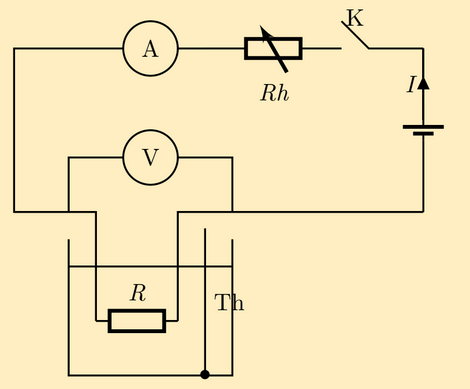
\includegraphics[width=0.3\textwidth]{./img/img_02.png}
\end{wrapfigure}


\subsubsection{Activité 2 :}
On réalise le montage électrique ci- dessous .
On met une masse de $m = 50g$ d’eau dans un bécher et on
introduit un conducteur ohmique de résistance $R = 2\Omega$ dans l’eau
de bécher .
\\On ferme le circuit et on règle le rhéostat afin que l’intensité du
courant atteint la valeur $I = 2A$, on mesure la tension $U_{AB}$ par un
voltmètre , on ouvre l’interrupteur , on agite et on relève la
température initiale $\theta$.
\\On ferme le circuit et en même temps on déclenche le chronomètre
à la date $t_0 = 0$. au bout de 2min , on note la température de l’eau
dans le bécher au cours de la durée $\Delta{t} = 2min$ et aussi l’intensité
du courant I = 4,8A et la tension $U_{AB} = 9,6V$

1.Calculer l’énergie électrique reçue par le conducteur
ohmique au cours de cette durée . : $W_e = U.I.\Delta{t} = 5.53kJ$

2.faire un rappel au loi d’Ohm . En déduire que l’expression
de la puissance reçue par le conducteur ohmique est la
suivante : $\mathscr{P}_e = R.I^2$

La loi d’ohm : $U=R.I$ donc $\mathscr{P}_e = U.I=R.I^2$

3.Calculer la quantité d’énergie thermique Q reçue par l’eau
de bécher .On donne :la capacité calorifique $\mu$ du bécher et l’eau est $\mu = 292Jk^{-1}$ et $\Delta{\theta} = 19^{\circ}C$

$ Q = \mu.\Delta{\theta} = 5.55Kj$

\subsubsection{Conclusion : }
Un conducteur ohmique est un dipôle passif  , il convertit toute
l’énergie électrique $W_e$ qu’il reçoit en énergie thermique $Q_j$ par
effet joule .
On désigne généralement l’énergie thermique $Q_j$ par $W_j$
et de ces deux relations $U_{AB} = R.I$ et $W_e = W_j = U_{AB}.I.\Delta{t}$ on
obtient la loi de Joule :
$$W_e = W_j = R.I^2.\Delta{t}$$

\subsubsection{Énoncé de la loi de Joule : }
\begin{tcolorbox}
\em{L’énergie électrique reçue par le conducteur ohmique et dissipée
par effet joule est proportionnelle au carré de l’intensité du
courant qui le traverse}
\end{tcolorbox}
\subsubsection{Conséquences de l’effet Joule : }
\begin{tcolorbox}
  L’effet Joule manifeste dans tous les récepteur parcourus par un
courant électrique , il est utile lorsqu’il constitue l’effet recherché (
fournir l’énergie thermique par chaleur ou par rayonnement
comme appareils de chauffage , éclairage par incandescence .. ) .
En revanche , il correspond une perte d’énergie dans le cas
contraire ( échauffement inutile dans des récepteurs qui peut
conduire à une détérioration de ces récepteurs , perte d’énergie
dans les lignes de transport d’électricité .. ).
\end{tcolorbox}

\begin{tcolorbox}[colback=black!15!white,
                  colframe=black!10!black,
                  title=Application 2 :
                 ]
On applique au bornes d’un conducteur ohmique de résistance
$R = 10\Omega$ une tension $U = 4V$.

  1. Calculer la puissance électrique reçue par la conducteur
ohmique . Sous quelle forme est convertie cette puissance ?

  2. Sachant que la tension U est appliquée pendant la durée
  $\Delta{t}$ = 5min.
Calculer l’énergie dissipée par effet joule .
\end{tcolorbox}

\section{Transfert d’énergie au niveau d’un
générateur : }
\subsection{Définition : }
Un générateur électrique est un dipôle actif qui convertit en
énergie électrique une autre forme d’énergie . 

Exemple : Une pile
\\- centrale thermique - centrale hydraulique - photopile .
Citer les formes d’énergies transférées pour ces générateurs .
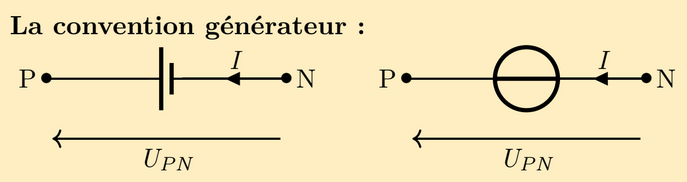
\includegraphics[width=0.5\textwidth]{./img/img_03.png}

La tension $U_{PN}$ est positive si le sens du courant électrique
de N vers P ou $U_{PN}$ et I ont même sens .

\subsection{Puissance et énergie fournies par un générateur}

a. La puissance électrique fournie par un générateur .
La puissance électrique fournie par un générateur au reste du
circuit est :
$$\mathscr{P}_e = \frac{W_e}{\Delta{t}} = U_{PN}.I$$
b. L’énergie électrique fournie par un générateur .
L’énergie électrique fournie par un générateur pendant la
durée $\Delta{t}$ , au reste du circuit est :
$$ 
W_e = U_{PN}.I.\Delta{t}
$$
\begin{tcolorbox}
Remarque : On note $W_e$ l’énergie électrique reçue par un dipôle,
$W_j$
l’énergie dissipée par effet joule et $W_u$ l’énergie utile
  \end{tcolorbox}

\begin{tcolorbox}[colback=blue!15!white,
                  colframe=blue!50!black,
                  title=Application 3 :
                 ]
Un générateur produit un courant électrique d’intensité $I = 3,14A$.

  1. Calculer la puissance électrique fournie au reste du circuit ,
sachant que la tension entre ces bornes est de $12,3V$ .

  2. Calculer l’énergie électrique fournie par le générateur durant
1 heure .

\end{tcolorbox}


\begin{tcolorbox}[colback=blue!15!white,
                  colframe=blue!50!black,
                  title=Application 4 :
                 ]
                 Pour préparer du dichlore ${Cl_2}_{(g)}$ par électrolyse d’une solution de
chlorure de sodium , on fait passer , dans une cuve à électrolyse ,
un courant de $35.10^3A$ ; la tension au bornes de la cuve est de
$U = 3,9V$ .

  1. Calculer la puissance électrique fournie à la cuve .

  2. Calculer l’énergie électrique fournie à la cuve fonctionnant
nuit et jours pendant 180 jours .On exprime cette énergie en kWh.

\end{tcolorbox}
\end{document}

